%五号字对应10.5pt,不知道这样设置对否?
\documentclass[10.5pt,twocolumn]{jbuaa}

%%画圆圈数字
\newcommand*\circled[1]{\tikz[baseline=(char.base)]{
            \node[shape=circle,draw,inner sep=1pt] (char) {#1};}}
            
%取消英文连词符
% \tolerance=1
% \emergencystretch=\maxdimen
% \hyphenpenalty=10000
% \hbadness=10000

\newcommand\mycolorRed[1]{{\color{red}#1}}
\newcommand\mycolorYellow[1]{{\color{yellow}#1}}
% \newcommand*\mycolorRed{\color{red}}

%%%????? 公式中字体的定义尺寸为 10 磅,上标/下标 68%,次下标/上标 42% ?????? 
\DeclareMathSizes{10.5}{10}{6.8}{4.2}
%%%% 本示例中带单位的数据采用的是siunitx来生成,好像默认与公式同样大小的字体,所以数字在正文中会小一些
%%%% 行文中普通数字大小为10.5pt,公式里或者用siunitx生成的数字则会是10pt,多少有点不协调。

%%%设置公式前后距离,差不多近似
\setlength{\abovedisplayskip}{2.5mm}
\setlength{\belowdisplayskip}{2.5mm}


\usepackage{tabu}
\usepackage{longtable}
\usepackage{makecell}
\usepackage{amsmath}
\renewcommand\cellgape{\Gape[-3pt][-3pt]}


%%%%%%%%%%%%%%%%%%%%%%%%%%%%%%%%%%%%%%%%%%%%%%%%%%%%%%%%%%%%%%%%
%      文章正文
%%%%%%%%%%%%%%%%%%%%%%%%%%%%%%%%%%%%%%%%%%%%%%%%%%%%%%%%%%%%%%%%
\begin{document}
%%%%%%%%%%%%%%%%%%%%%%%%%%%%%%%%%%%%%%%%%%%%%%%%%%%%%%%%%%%%%%%%
% 标题,基金项目,作者,通信地址定义
%%%%%%%%%%%%%%%%%%%%%%%%%%%%%%%%%%%%%%%%%%%%%%%%%%%%%%%%%%%%%%%%
\title{
\vspace{1cm} \erhao\hei 水翼艇原理与设计 \vspace{-0.2cm}
}

\author{
\sihao\fang 简心语 \makebox{$^{\text{1}}$}\\[0.1cm]
\liuhao (1.~~上海交通大学~~船舶与海洋工程学院,上海~~200240) 
}

\date{}  % 这一行用来去掉默认的日期显示
%%%%%%%%%%%%%%%%%%%%%%%%%%%%%%%%%%%%%%%%%%%%%%%%%%%%%%%%%%%%%%%%
% 奇数页页眉
%%%%%%%%%%%%%%%%%%%%%%%%%%%%%%%%%%%%%%%%%%%%%%%%%%%%%%%%%%%%%%%%
\fancyhead[CO]{{\footnotesize 简心语: 水翼艇原理与设计}}            %请在这里写出第一作者以及论文题目
%%%%%%%%%%%%%%%%%%%%%%%%%%%%%%%%%%%%%%%%%%%%%%%%%%%%%%%%%%%%%%%%
%%%%%%%%%%%%%%%%%%%%%%%%%%%%%%%%%%%%%%%%%%%%%%%%%%%%%%%%%%%%%%%%
%  显示title,并设页码为空(按杂志社要求)
%%%%%%%%%%%%%%%%%%%%%%%%%%%%%%%%%%%%%%%%%%%%%%%%%%%%%%%%%%%%%%%%
%%%%%%%%%%%%%%%%%%%%%%%%%%%%%%%%%%%%%%%%%%%%%%%%%%%%%%%%%%%%%%%%
%      中文摘要
%%%%%%%%%%%%%%%%%%%%%%%%%%%%%%%%%%%%%%%%%%%%%%%%%%%%%%%%%%%%%%%%
\CKeyword{水翼艇; 水翼; 水动力学; 展望 }
\CLCNo{XXXX\makebox{$^{\scalebox{0.6}{\!+}}$}.X;XXXXX}
\Dcode{A}
\PaperNo{0000-0001 (XXXX) XX-XXXX-XX}

\twocolumn[
  \begin{@twocolumnfalse}
  \maketitle

\begin{CAbstractJBUAA}
本文对水翼艇做了总体的概述。首先介绍了水翼艇的的概念及其详细的发展历史。继而对水翼的水动力学研究现状做了简要总结,并举例说明有限元方法在水动力学分析中的应用。然后在简化条件下,对水翼的原理作定量的分析,首先扼要介绍了水翼的几何特征和水动力特征,接着分析了升力来源,最后详细介绍了阻力的成因和计算。接着简要介绍了水翼艇的各种类型。最后从应用(军用和民用)和限制两个方面,展望了水翼艇的未来。
\end{CAbstractJBUAA}

%%%%%%%%首页角注
\positiontextbox{2.0cm}{25cm}{
\noindent\rule{4cm}{.5pt}\\[0.5ex]%
\hspace*{1em} \liuhao \linespread{0.8}\selectfont
\parbox{\textwidth}{%
\hei\makebox[\widthof{\makebox{*}收}][r]{收}稿日期: 2017-12-12; 录用日期: 2017-12-12;\\
\hei\makebox[\widthof{\makebox{*}收}][r]{基}金项目:国家自然科学基金(基金号~12345678)
}}
  \end{@twocolumnfalse}
]


%%%%%%%%%%%%%%%%%%%%%%%%%%%%%%%%%%%%%%%%%%%%%%%%%%%%%%%%%%%%%%%%
%  正文由此开始-------------------------
%%%%%%%%%%%%%%%%%%%%%%%%%%%%%%%%%%%%%%%%%%%%%%%%%%%%%%%%%%%%%%%%
%%%%%%%%%%%%%%%%%%%%%%%%%%%%%%%%%%%%%%%%%%%%%%%%%%%%%%%%%%%%%%%%
\wuhao 
%  分栏开始

%%%%%!!!!!正文在第一页两栏分别合适位置插入 \enlargethispage{-3.3cm},给首页跨双栏脚注留空间,大小需要结合前面位置和高度手动设置!!!!!
%%%%%%%%%%%%%%%%%%%%%%%%%%%%%%%%%%%%%%%%%%%%%%%%%%%%%%%%%%%%%%%%

自船舶诞生之初,高速性一直是船舶工程师们的追求,而传统的单体排水船型经过长期研究已经到达瓶颈,难以产生新的突破。因此人们开始寻求各种新船型,甚至颠覆原有的推进方式,来使舰艇性能得到巨大改善。在这些高性能船型中,水翼艇发展较早,并以其高速性和适航性等特点得到快速发展,并广泛应用于军事和民生。

对于传统船型,在高速的情况下,兴波阻力将占船体总阻力的40 \%-50 \%,摩擦阻力约占50 \%,粘压阻力仅占5 \%左右。另一方面,摩擦阻力约略正比于速度的平方,而兴波阻力约略正比于速度的六次方。由此可见,若能减小兴波阻力,舰艇速度将能大大提高,水翼艇正是基于这种考虑。顾名思义,水翼艇就是有在在水中工作或割划水面的机翼,像飞机机翼一样,产生一定的升力,一旦船舶达到一定速度,升力将使船体离开水面,极大减小了湿表面积,消除了船体带来的兴波阻力,只有水翼支架和水翼与水接触,故而使高速航行是的总阻力大为减小。\enlargethispage{-3.3cm}并且因为水的密度较空气的密度约大八百余倍,在同等升力之下,水翼的尺度比机翼小得多。靠水翼升力支持艇重的水翼艇比滑行艇阻力小,兴波小,受波浪干扰影响也小,因而具有良好的快速性和适航性。\enlargethispage{-3.3cm}


\section{水翼艇的发展}
水翼艇的设想由来已久 , 可能自飞机问世便出现在工程师们的脑海中。早在1891年,一个名叫兰伯特的法籍俄国贵族在一艘小艇上加装滑水板,使得小艇在航行是受滑水板的作用略有抬起,船体所受阻力降低,速度明显提高。这便是水翼艇的萌芽了,一如诸多伟大发明,诞生于无意的尝试中。二十世纪初,汽车与飞机工业的发展促进了重量轻、马力大的发动机生产,从而为高性能船的发展埋下伏笔。1906年,意大利人福兰尼尼和克罗科在小艇上假装了四个梯形水翼,航速最终达到90km/h。同年美国人麦克莫发表关于水翼原理的文章。电话的发明人贝尔与鲍德温合作建造,最终在1919年9月创下时速114公里的纪录。然而由于那个时代正是水上飞机、滑行艇发展的摇篮时代,水翼技术更多地被用于研究如何帮助水上飞机起飞,加之当时水翼艇在理论和实践方面仍存在不少问题,故之后其发展几乎处于停滞状态。直到1934年,苏联学者弗拉季米罗夫发表水翼动力学理论和水翼兴波阻力计算方法,奠定了水翼艇发展的理论基础。

1935 年,德国发展建造了割划 V 型水翼艇,航速达 30 kn。苏联在 五十年代,由阿列克塞耶夫主持开发了内河水翼艇“火箭”号等 , 以浅全浸水翼为主自成系列,自 1957 年先后建成12个型号的水翼艇并投入使用,其中大多为割划自稳式和自稳自控式水翼,营运速度可达37 kn。美国也是水翼艇发展大国之一,其研发的全浸自控水翼客艇采用喷水推进装置,该项技术得到其他国家的广泛认可和采纳。九十年代初,日本的日立、三井和三菱等公司分别进行了水翼艇的设计研究,其中多以铝合金制造减轻船体质量,采用喷水推进或柴油机推进增大推进动力,并不断改进,采用计算机控制系统提高耐波性和适航性,最大航速在40 kn 左右,载客量达几百人,并投入到航运中。2002 年,俄罗斯研发的双体水翼船航速达到50 kn,成为世界上最快的船舶之一。2003 年,美国研究了托升船体型双体水翼艇,2006 年 BLB-70 模型下水,艏部安装托升体,起到了球鼻艏的作用,可有效减小兴波阻力。2010 年,俄罗斯恢复对水翼艇的建造,开始设计新型复合、大吨位水翼艇,预计到2020年吨位达到千吨级。自此,新型水翼艇吸引了很多学者和企业的眼球。

我国发展起步相对国外较晚,于1959 年建造了第一艘水翼客艇“水翼一号”,这是我国在水翼艇发展上的突破。其后,我国又发展了自稳加自控式水翼艇,1970年建造了使用自控系统的101试验艇,并采用能量谱分析法对系统进行调试。1988 年我国自行研制建成第一艘全铝焊接的水翼小客艇“飞鱼”号,是我国水翼艇发展从科研阶段进入工程应用阶段的重大进步。 九十年代,上海交通大学对小水线面和割划式混合水翼艇进行了研究,理论和试验结果表明,其航行阻力和稳定性较好。2005 年,中国船舶科学研究中心设计建造了我国第一艘混合水翼双体船,其在波浪中航行的阻力和横摇响应大大减小。2014 年,赵熊飞等对高速复合型水翼船运动特性进行研究,取得了较大的进展。我国的许多学者对水翼的构型如何影响水翼艇航行、水翼水动力参数的求解以及水翼艇的自动控制装置等方面进行了相关研究。

%引言不编排节号,不插图列表。引言应说明课题的背景,引述该领域的国内外同行已经取得的进展,突出本研究工作的选题意义和创新点\citeBUAA{Harpold1979Shuttle,Yu2011Guidance}。内容不应与摘要和结论雷同\citeBUAA{Hu2015Steady}。在论述本文的研究意义时,应注意分寸,切忌使用“有很高学术价值”、“填补了国内外空白”、“首次发现”等不适之词;同时也注意不要使用客套话,如“才疏学浅”、“水平有限”、“恳求指教”之类的语言\citeBUAA{Laning1956Random,Zarchan2013Tactical,Zadeh1963Linear}。

\section{水翼的水动力学研究进展}
经过近半个世纪的研究,水翼的水动力学理论从最初的二维,发展到更贴实际情况的三维,并考虑水面兴波的影响和粘性的影响。研究方法也从最理想化的理论模型分析模型发展到现在的水池试验和数值模拟。

水翼的水动力学研究始于上世纪60年代,Giesing和Smith\cite{giesing}通过二维定常移动源自由表面格林函数的推导和计算,结合势流边界元理论,发展了二维定常水翼升力理论。戴遗山等人\cite{dai}利用偶极子分布法结合自由表面格林函数研究了三维水翼的兴波问题。Bal等人\cite{bal}\cite{bal2}利用Rankine源方法,研究了二维和三维近自由表面空化水翼的升力性能,在自由表面上采用四阶差分格式保证数值稳定。黄胜等人\cite{huang}采用多目标粒子群算法对水翼剖面进行了优化。鲁传敬和何友声\cite{lu}将三维水翼简化为一个涡环,采用时域格林函数分析了三维水翼的升为性能。张利军和王言英\cite{zhang}采用B样条的边界元理论建立了三维水翼水动力性能的预报方法,重点对翼梢和尾涡进行了研究。李国安和叶恒奎\cite{li}采用时域格林函数研究了带有水翼的船体的兴波问题,水翼采用升力线模型来表达。陈庆任等人\cite{chen}利用时域Rankine源法对近自由表面三维非定常振动水翼进斤数值分析,并对不同振动频率下计算出升力,阻力等水动力学参数进行了计算。Faltinsen和Semenov\cite{fal}利用保角变换,研究了二维局部空化的水翼,同时也考虑了自由表面的非线性。

随着计算流体动力学的发展,对水翼进行数值模拟己经成为可能。程闻等\cite{cheng}利用有限元法求解雷诺平均的NS方程研究了粘性流体中二维水翼的非稳态空化问题。胡世良等人\cite{hu}利用有限元法研究了三维水翼的水动力学性能,并考虑了水翼的弹性变形。谢宜和郑义\cite{xie}采用有限元及RNG $k-\epsilon$湍流模型对粘性流体中二维和三维近水面航行的水翼进行了数值模拟,并发现升力的强非线性现象。

下面就以胡世良等人\cite{hu}的工作对新兴的数值方法做简要介绍。他们首先构建数学模型,继而选择采用基于紧耦合的算法,最后结合有限体积法(FVM)与有限元法(FEM),模拟了水洞中三维悬臂水翼的流固耦合运动。水翼一端固定在水洞壁面上,另一端则是自由的,将水翼视作刚性体,在水翼附近的流场网格采用了楔型体网格,而水翼则用20节点六面体有限单元离散。构建好的模型参见图\ref{fig:cfd1}、图\ref{fig:cfd2}。计算结果表\ref{tab:1}所示,可以看到数值解与实验值之间的误差随着网格数的增加而减少。而网格数为$7 \times 1{0^5}$时误差仅为0.42\%。
\begin{figure}
	\centering
	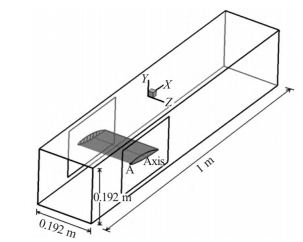
\includegraphics[scale=1,trim=0 0 0 0]{image/cfd1}
	\caption{流场计算域示意图}
	\label{fig:cfd1}
\end{figure}
\begin{figure}
	\centering
	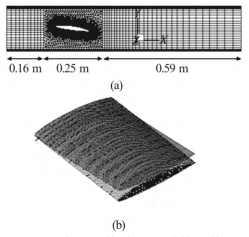
\includegraphics[scale=1,trim=0 0 0 0]{image/cfd2}
	\caption{流场网格截面及结构网络}
	\label{fig:cfd2}
\end{figure}

\begin{table}[h]
	\centering
	\begin{tabular}{l c r}
		\hline
		& $C_L$ & 误差\\
		\hline
		Coarse($4 \times 1{0^5}$) & 1.188 & 0.59 \% \\
		\hline
		Middle($7 \times 1{0^5}$) & 1.186 & 0.42 \% \\
		\hline
		Fine($9 \times 1{0^6} $) & 1.185 & 0.54 \% \\
		\hline
		Experiment & 1.181 & 0\\
		\hline
	\end{tabular}
	\caption{不同网格数计算得到的升力系数与实验值比较}
	\label{tab:1}
\end{table}



\section{水翼的原理}
%\enlargethispage{-3.3cm}
%题目应简洁、准确,能恰如其分地概括研究的范围和深度,避免使用希腊字母和上下标。英文题名中第一个单词首字母大写,其余小写(专有名词首字母大写)\citeBUAA{Weiss2005Adjoint,Zarchan1979Complete,Weiss2005Handover}。
%
%作者署名及署名排序应协商一致。姓名的英译采用汉语拼音,姓前名后,姓全大写,名首字母大写。如:ZHANG Ying(张颖),WANG Xilian(王锡联),ZHUGE Hua(诸葛华)。
%
%通讯作者一般为导师或课题负责人。
%
%单位应为论文首次投稿时的作者所在单位。单位的著录一般应到系一级,单位应著录全称,单位名称的英译应统一正确\citeBUAA{Lin1996ResearchAdjoint,Zou2001Adjoint}。

\subsection{水翼的几何特征及水动力特征}
水翼是在水中运动时能产生升力并用于支撑艇重的翼形结构。一副水翼一般由产生升力的翼板、翼板与艇体间连接的支柱及其他附件组成。水翼的升力特征,主要取决于翼板的几何特征,由水翼的弦长、翼展、展弦比、平面形状、前视形状和翼剖面形状等几何要素来表征。。水翼的平面形状有矩形、后掠形、菱形和两端加宽形等。翼剖面形状有平凸弓形、凹凸弓形、机翼形等。水翼的前视形状有V 形、梯形、平翼等。按作用原理和结构形式可分为全浸式、割划式、浅浸式、深浸式、阶梯式、分离式、后掠式水翼和无空泡、全空泡、过渡空泡、通气、供气、可收、可控水翼等,水翼多用高强度、重量轻的材料制造。水翼的水动力特性与其几何要素(攻角、相对浸深、空泡数、傅汝德数和雷诺数)有关,在很大程度上决定了水翼艇的性能。

水翼两个翼梢之间的距离,称为翼展(span),水翼沿来流方向的截面称为翼剖面,其长度称翼弦。翼梢处的弦长称为梢弦(tip chord),翼根处弦长称为根弦(root chord),两者的比值为尖削比(taper ratio)。对于尖削比不等于1的水翼,要通过计算求出其平均弦长,计算方法是用水翼平面形状的面积除以翼展。翼展与平均弦长的比值称为展弦比(aspect ratio)。展弦比越小,翼的三维效应就越大,反之,当展弦比趋于无穷大时就成了二维问题。翼剖面又称为翼型,在水翼设计上已经有了像螺旋桨一样的系列图谱,工业设计翼型如美国的NACA翼型、苏联的UArK翼型及德国的G6ttingen翼型等,理论翼型如儒可夫斯基翼型和和卡门—脱里夫茨翼型等。

流体的作用力包括垂直于水翼表面的水动压力以及切向力,这些力合成为水动力主向量P和水动力主力矩M。如\ref{fig:force}所示,主向量在运动方向和垂直方向的投影分别为水翼的阻力R和升力L。水翼的主要水动力特征参数为升力系数$C_L$、阻力系数$C_R$、力矩系数$C_M$和升阻比$K$.
\begin{figure}
	\centering
	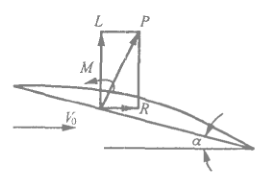
\includegraphics[scale=1,trim=0 0 0 0]{image/force}
	\caption{水翼剖面受力图}
	\label{fig:force}
\end{figure}

\subsection{水翼的升力}
为简化问题,将水翼在水中作匀速直线运动视作均匀来流问题。根据伯努利方程,由于水翼上下表面的不对称,使得上表面流速大,相应压力小;下表面流速小,相应压力大。水翼上下表面的压差构成了水翼的升力。
假设流体无黏且有势,有限翼展水翼升力系数为
\begin{equation}
\label{cl}
C_L = \alpha_{\infty}(\alpha - \alpha_i + \alpha_0)
\end{equation}
式中,$\alpha_{\infty} = \dfrac{dC_L}{d_{\alpha}}$是二元机翼升力系数曲线的斜率。$\alpha$是冲角,如图\ref{fig:force}所示。$\alpha_i$是下洗角,由于翼端的存在,翼两端下表面处于高压区的水流有向上表面低压区流动的趋势,使水翼附近的水流产生了一个向下的诱导速度$v_i$,它与原来的来刘速度回合,相当于使来流偏转了一个角度$\alpha_i$,成为下洗角,如图\ref{fig:downwash}所示。$\alpha_0 = -2\dfrac{f}{c}$是零升力角,其中$f$为水翼拱度,$c$为弦长。由此可见,下洗角是求出的升力系数的关键。
\begin{figure}
	\centering
	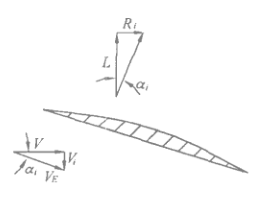
\includegraphics[scale=1,trim=0 0 0 0]{image/downwash}
	\caption{有限翼展水翼的下洗}
	\label{fig:downwash}
\end{figure}
下洗角与机翼的平面形状有关。当翼的平面形状是椭圆型时,其升力沿展长方向也是椭圆分布,此时下洗角为
\begin{equation}
\label{downwashangle}
\alpha_i = \dfrac{C_L}{\pi A}
\end{equation}
对非椭圆形状,可用系数修正。此外,实际环境必须考虑水的粘性,一般用系数0.87\~{}0.90进行修正。

\subsection{水翼的阻力}
水翼的总阻力为翼型阻力、兴波阻力和诱导阻力的总和。
\subsubsection{翼型阻力$C_V$}
由流体黏性引起的,包括摩擦阻力和形状阻力。
水翼摩擦阻力的大小取决于边界层内流动的状态,后者可用雷诺数$Re = \dfrac{vl}{\nu}$表征,其中$l$取水翼弦长$c$,根据雷诺数的不同取不同计算公式。
\begin{equation}
{C_f} = \begin{cases}
\frac{{1.327}}{{\sqrt {Re} }},                                           Re < 3 \times 1{0^5}\\
\frac{{0.455}}{{lgR{e^{2.58}}}} - \frac{{1700}}{{Re}} , 3\times 1{0^5} < Re < 1{0^7}\\
\frac{{0.455}}{{lgR{e^{2.58}}}}or\frac{{0.075}}{{{{(lgRe - 2)}^2}}},     Re > 1{0^7}
\end{cases}
\end{equation}
当边界层的流动状态为紊流时,即$Re>1{0^7}$时,需考虑水翼表面粗糙度的影响,一般取粗糙度补贴$\delta C_f = 0.8 \times 1{0^7} $。也可用NACA的标准粗糙度机翼试验结果整理得到的摩擦阻力系数公式:$ C_f = 0.08Re^(-\dfrac{1}{8})$而无需再考虑粗糙度补贴。

在粘性流体中,由于粘性损耗翼剖面后部的压力比理想流体要小,造成压差阻力。这个阻力主要取决于翼剖面形状,故被称作形状阻力。
\begin{equation}
C_p = 2C_f(1.2\overline{e} + 60\overline{e}^4)
\end{equation}
式中,剖面的相对厚度$\overline{e}=\frac{e}{c}$,$e$是翼剖面的最大厚度,$c$是弦长。

\subsubsection{诱导阻力$C_D$}
回顾前述的下洗角图\ref{fig:downwash},翼端绕流相当于使来流向下偏转了角度$\alpha_i$,使通过水翼的来流速度由原来的$V$变为$V_E$。这时作用在水翼上的水动力除升力$L$外,还有与来流方向相反的$R_i$,称之为诱导阻力。诱导阻力与升力同时产生,随升力增加而增加。其还与水翼的展弦比及平面形状有关,平面形状为椭圆的机翼诱导阻力系数为
\begin{equation}
C_D = C_L\alpha_i=\frac{C_L^2}{\pi A}
\end{equation}
对于其他形状的机翼,可添加修正系数。

\subsubsection{兴波阻力$C_W$}
自由表面的存在导致兴波阻力。首先介绍浸深的概念,水翼浸深常指水翼压力面1/4弦线处至自由表面的距离,记为$h$。行波阻力系数可表示为
\begin{equation}
C_w = \frac{C_{L\infty}^2}{2Fr_c^2}[1-\frac{2\pi}{Fr_c^2}]
\end{equation}
式中,$C_{L\infty}$是无限浸深水翼的升力系数,$Fr_c^2=\frac{v}{\sqrt{gc}}$是水翼弦长傅汝德数。




\section{水翼艇的分类}
如图\ref{fig:class},水翼艇按水翼数量的多少,分为单水翼艇(只有前水翼,又称翼滑艇)和双水翼艇(前后水翼)两种,单水翼艇艏部一般通过浅浸水翼支撑艇体,尾部为滑行面,双水翼艇则利用前、后两个水翼支撑艇体航行,双水翼艇可以实现翼航状态;按水翼攻角可否调节,可分为自控和非自控(固定)两种;按翼航时水翼是否穿越水面,分为割划式、全浸式和浅浸平翼式;按艇体是否拖出水面可分为普通式和全浸式;双水翼按前后水翼载荷分布可分为鸭式、飞机式和串列式。
\begin{figure}
	\centering
	\includegraphics[scale=1,trim=0 0 0 0]{image/class}
	\caption{水翼艇的分类}
	\label{fig:class}
\end{figure}

最为常见的划分方式还是按翼航时水翼是否穿越水面,下面就此详细介绍。
水面割划式水翼在航行时有一部分露在水面之上,仅部分面积浸没在水中,它依靠改变水翼浸水状况来调节水翼升力,而不需要其他附属设备。因此结构简单,使用可靠。水面割划式水翼艇的优点是自稳性好,储备水翼面积大,进入翼航状态速度低等。它的缺点是对波浪扰动比较敏感,在波浪中不容易维持稳定的升力,不适宜在风浪较大的海域高速航行。

全浸式水翼艇的结构特点是水翼全部浸沉在水中,艇体由连接水翼的垂直支柱支撑。全浸式水翼艇按照水翼浸深的不同,可分为浅浸式和深浸式。水翼浸水深度小于水翼弦长的称为浅浸式,深于弦长的为深浸式。浅浸式水翼艇利用水翼浸水深度的变化来控制艇体的稳定,因为水翼浸水深度不大,当艇体发生倾斜时,一侧水翼可能被抬出水面,产生的升力减小;而浸水深度大的一侧水翼则产生比另一侧更大的升力,以这一方式所形成的回复力矩将倾斜的艇体扶正。割划式水翼的平衡原理与浅浸水翼大致相同,都是利用两侧水翼的升力差异产生的回复力矩来扶正艇体,浅浸式水翼艇和割划式水翼艇都具有自稳性,而深浸式水翼艇的水翼所产生的升力不会因为水翼浸水深度的改变而改变,这个特性使得深浸式水翼艇能在一定风浪条件下平稳高速航行时不具备自稳性的功能。深浸式水翼艇水翼升力的调节主要是通过自动控制系统控制水冀的攻角或调节水翼后缘襟翼的攻角等来实现,以此来维持深浸式水翼艇航行过程中的稳定。

\section{展望}
\subsection{军事应用}
跟其他的高速舰艇技术相比,水翼船(主要是全浸型)的主要优点是能够在较为恶劣的海情下航行,船身的巅簸较少,而且高速航行时所产生的兴波较为少,对岸边的影响较低。这一点在军事上应用前景广阔,尤其是对于机动性和适航性要求高的近海登陆作战,这也是在六十年代各国纷纷研制水翼艇的原因。
\subsection{客运市场}
水翼艇是目前世界上建造最多,正在营运最多的高速客艇,据统计,水翼艇总数约为其他所有高速船总和的2\~{}3倍。显然,水翼艇在世界高速客运中的地位不容忽视。由于水翼艇的小阻力性,水翼艇的经济航速处于55\~{}95km/h之间,且失速非常小。运动性能对比后表明,水翼艇的运动加速度最小,纵摇亦最小;另一方面,高速航行是水翼艇不会受到波浪的直接冲击,耐波性非常好,例如110吨的Jetfoil全浸自控水翼艇可翼航于3.5m浪高,是世界公认耐波性最好的高速客船。所以,水翼艇带给乘客的体验相对来说是很舒适的。我认为,客运中最重要的三个指标是安全、快速、舒适,而这三点,水翼艇全部满足。而且,水运比之陆运、空运是投资最少的运输方式。目前我国在水运方面仍以低速排水型船为主,费时费力。2015年我国水路客运量2.71亿人、旅客周转量73.08亿人公里。若按现有的平均速度为30km/h左右,能有十分之一的乘客换乘水翼艇,航速提高30km/h左右,则能节省约51万个工作日,能增加多少经济效益!
\subsection{限制}
缺点主要在制造大型的水翼船、或进一步提高速度,目前还存有技术困难,现今存在的水翼船大多不超过1000吨,并以近海航行为主。水翼所能提供的浮力与长度成平方关系,但是船的重量却与长度成立方的关系(平方/立方定律)。但其实推进问题在大型化中更加难以解决,因为水翼艇水下部分很小,无法安置发动机在水下。另一方面,要进一步提高速度,水翼在高速下会产生气泡的问题亦需要解决。此外全浸式水翼的结构及控制较为复杂,亦令成本上涨。水翼船使用燃气引擎花费燃料较多亦是商业运作上的考虑之一。
\subsection{一点结论}
综合上述三个方面,我认为水翼艇本身在技术上的壁垒很强,今后的发展空间不大,除非人类在推进系统、材料、水动力学上有重大突破;但在应用方面尚有广阔的空间,包括军用和民用,若能进一步推广,将给人们的出行带来便利,产生巨大的社会经济效益。不过,换个思路,水翼的原理可巧妙用在其它方面,比如用于改进小水线面船、大型气垫双体船等高速船的性能。











%\section{正文}
%\subsection{量、单位、公式}
%\subsubsection{公式编排}
%\label{labSecForm}
%《北京航空航天大学学报》一般不编排单独的符号表,对于公式中的变量含义需要说明的,请在公式后的段落中,采用``式中:$A$为某某;$B$为某某;……"的方式加以说明。
%\begin{equation}
%\label{eqnLabelp}
%p_1 (h) = \dfrac{n_{\textnormal{He}}RT}{V}-\rho_{\textnormal{He}}gh
%\end{equation}
%式中:$n_{\textnormal{He}}$ 和 $\rho_{\textnormal{He}}$ 分别为艇囊内部氦气的物质的量和氦气在温度 $T$ 时的平均密度;
%$V$=\SI{36893.426}{\cubic\meter}%%数字会小一些,默认的是公式字体大小
%为艇囊体积;$T$=\SI{216.65}{\kelvin}为艇囊内稳态温度;$h$为距离艇囊中心轴线($x$轴)的垂直高度.请使用Mathtype编辑。公式中字体的定义尺寸为10磅,上标/下标68\%,次下标/上标42\%,符号150\%,次符号100\%(设置方法:Mathtype-尺寸-定义)。长公式如需转行,应在记号=,+,$-$等之后断开,而在下一行开头不再重复这一记号。
%
%\subsubsection{量和单位}
%有关记号的使用应符合国家标准,例如:$\sin^{-1}$应为$\arcsin$,$\rm ctg$应为$\cot$,$\rm tg$应为$\tan$,不要使用非国家法定单位,如ppm等表示法已要求停止使用(rpm应写为r/min);除$Re$, $Ma$(其中$e$, $a$不是下标)等几个特征数外,变量应使用单个字母表示,可以带上标和下标(否则由多个字母表示单个变量,易被误解为多个变量相乘)。
%
%\subsubsection{字体}
%矩阵、向量请用粗斜体表示,变量用一般斜体表示;下标字母若为说明性的(如英文缩写)则用正体表示,若为量和变动性数字及坐标轴的符号则用一般斜体表示(设置方法:Mathtype-样式-定义-高级)。
%
%所有文中出现的符号请另附文档说明其是变量、向量等,并说明各变量上下标的含义,以便编辑确定它们应采用的排版字体(变量符号说明表)。
%
%请作者对易于混淆的字母和数字,如数字0和字母o,英文a和希腊字母$\alpha$,O,P,S,C等的大小写,批注``英大"(代表英文大写)、``数字0"、``希小"(代表希腊字母小写)等。
%
%\subsection{图、表}
%图、表需给出中英文图题、表题(子图也需给出图题),但图表中图例、线型说明等一律用中文。图表一般不超过7.7\ cm宽。金相图和计算机云图,其中的比例尺等字编辑过程中都不再重贴,按照照片处理,如有这两类图请保证美观清晰,字体用times new roman。
%
%\subsubsection{图片}
%对于函数曲线图,采用全框图,并注意检查以下各项:
%
%1)横纵坐标的标目(即变量名),尽量使用国标变量符号,变量名要在正文中交待,且与正文中符号一致;若正文中无,也可使用中文名称。
%
%2)坐标轴标目的量纲,对于无量纲化或无单位的,请注明``无单位”。
%
%3)坐标轴上的刻度线朝内,刻度值完整(坐标轴始末点均应有完整刻度值)。
%
%4)不同线型或图符是否有说明。
%
%5)是否矢量图格式,从软件中输出或拷贝矢量图格式直接插入文档中,避免用拷屏办法插图图片,否则后期无法编辑。
%
%6)类似图片尺寸尽量相同。
%
%《北航学报》自2014年起可提供彩版印刷,如有彩印需求请作者在“出版工作单”中注明。若不需彩印,请作者作图时注意用可区分的线形或符号区分不同曲线,以保证黑白图清晰可分辨。 
%
%图中文字均用中文或变量名称表示!
%\begin{figure}[b!]
%\centering
%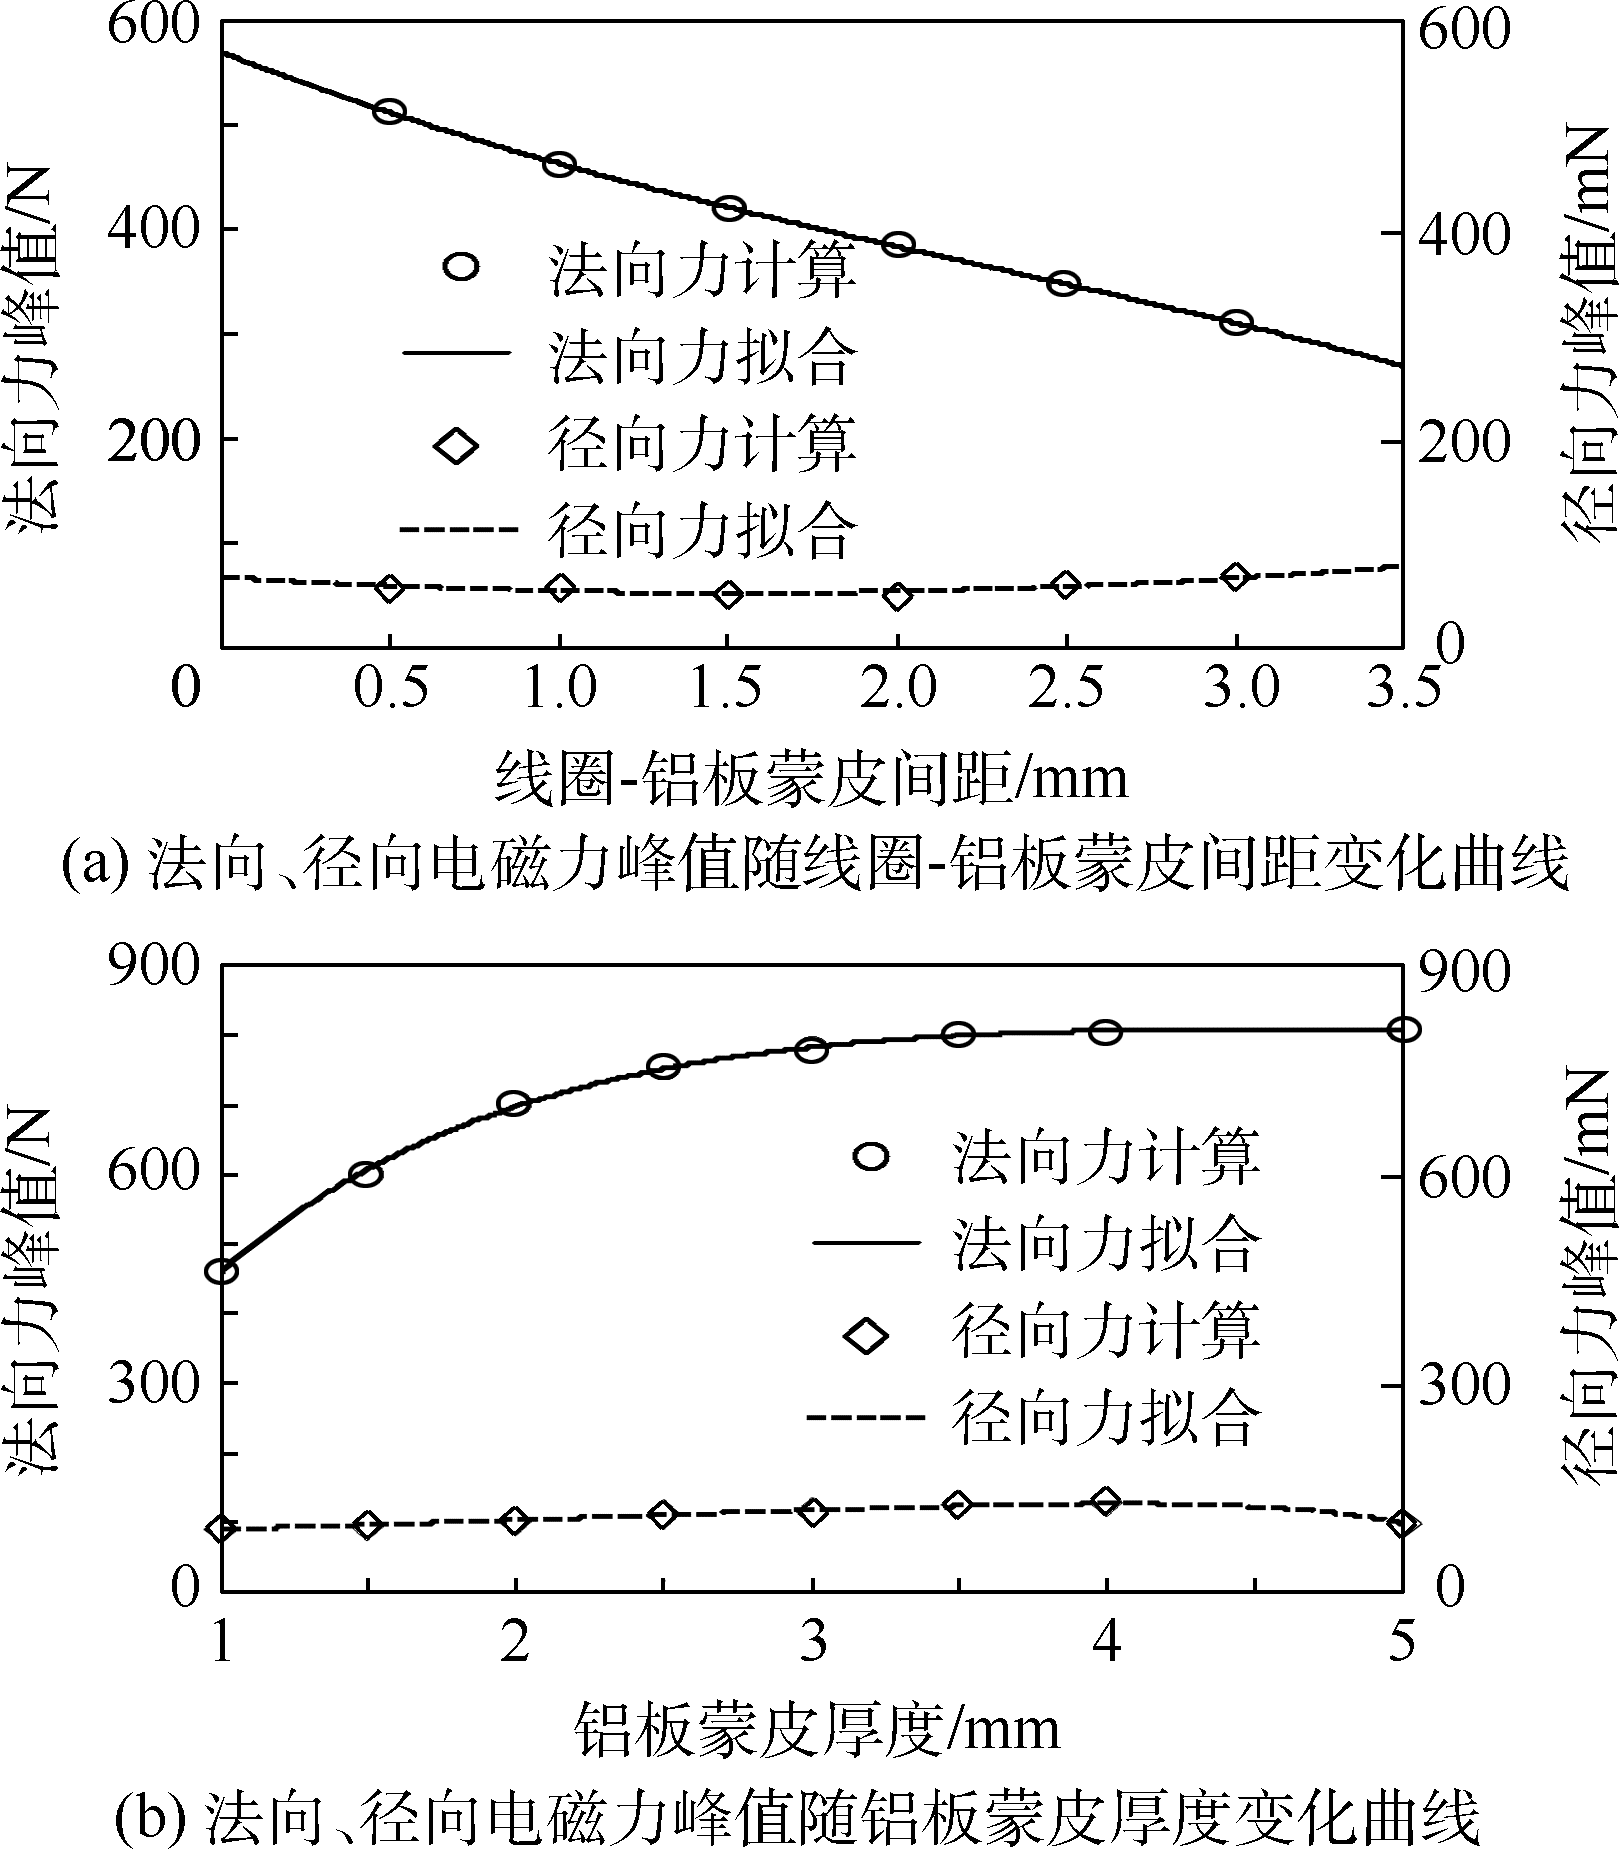
\includegraphics [scale=1,trim=0 0 0 0]{./image/tu1.png}
%\bicaption[labelFigtu1]{图}{\centering 电磁力峰值随线圈-铝板蒙皮间距和铝板蒙皮厚度变化曲线}{Fig.}{\centering Curves of electromagnetic force peak changing with coil-aluminum-plate gap and thickness of aluminum plate}
%\end{figure}
%
%图片样例见图\ref{labelFigtu1}和图\ref{labelFigtu2}(目前是位图格式,不能编辑,作者应提供可编辑的矢量图)。
%
%\begin{figure}[h!]
%\centering
%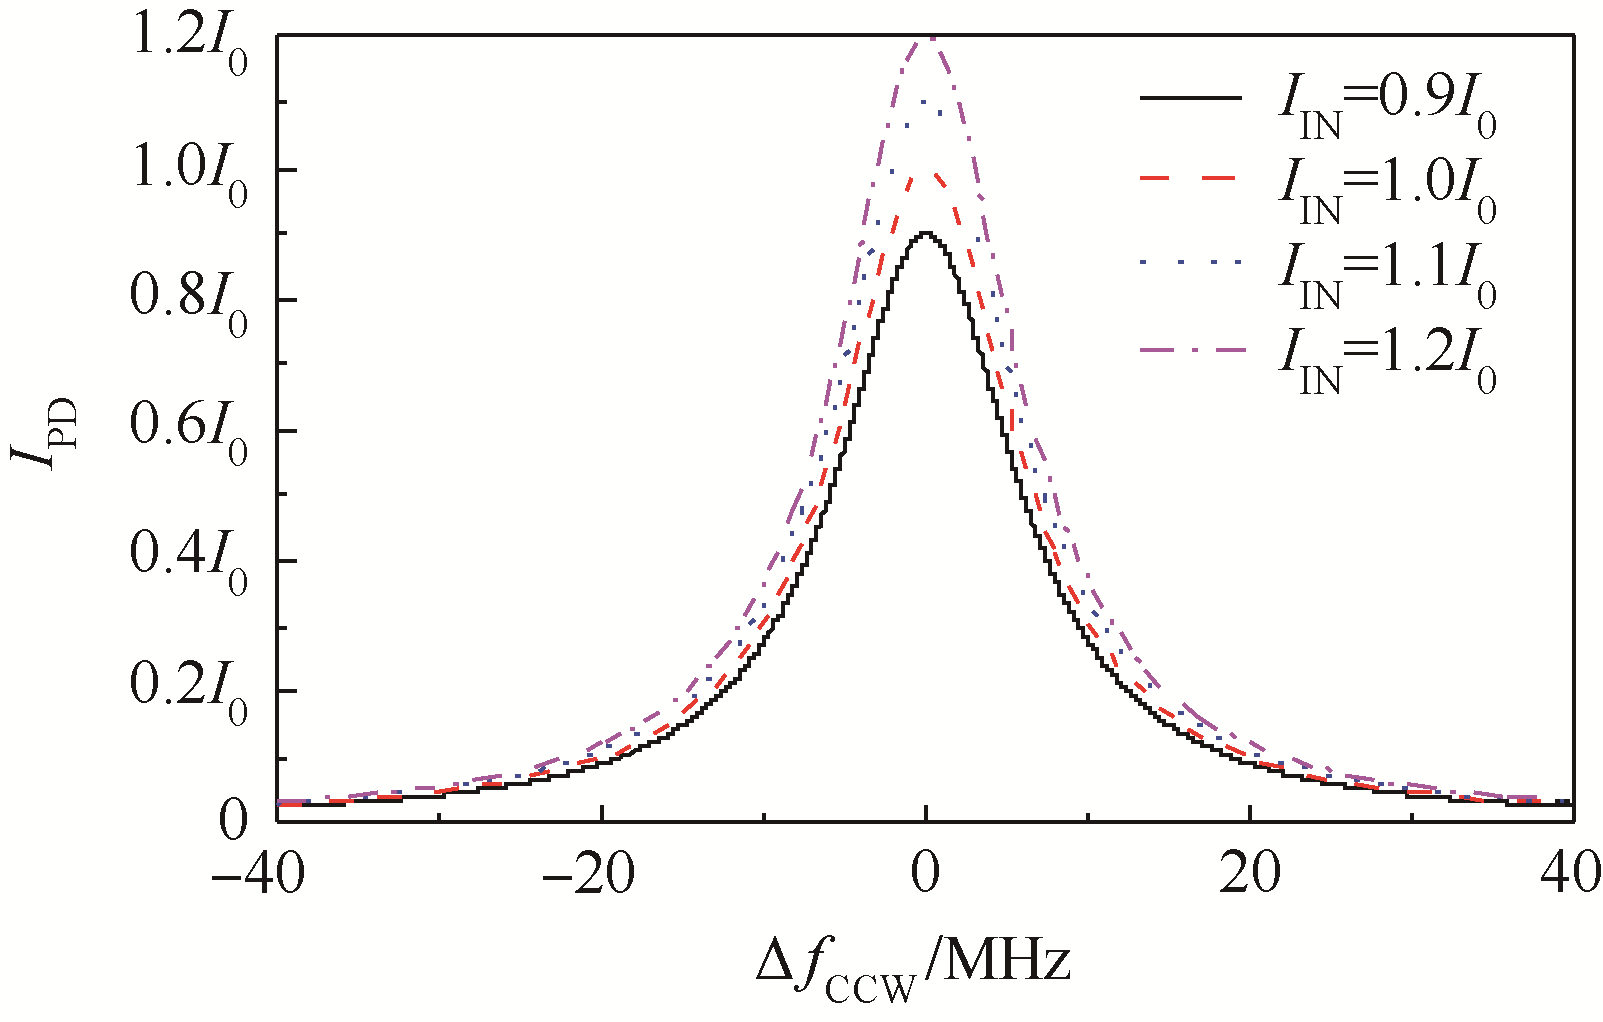
\includegraphics [scale=1,trim=0 0 0 0]{./image/tu2.png}
%\bicaption[labelFigtu2]{图}{\centering 谐振腔输入光强波动对谐振曲线的影响}{Fig.}{\centering Fluctuation influence of the resonator's input intensity on resonance curve}
%\end{figure}
%
%\subsubsection{表格}
%请使用三线表。选中表格,点右键打开``边框和底纹”,可对表格的边框等格式进行编辑,三线表的一般格式见表\ref{labelTabtab1}。
%\begin{table}[h]
%\centering
%\captionnamefont{\xiaowuhao\bf }
%\captiontitlefont{\xiaowuhao\bf }
%\bicaption[labelTabtab1]{表}{传输线积冰条件}{Table}{Icing conditions of transmission line}
%\renewcommand\tabcolsep{1em}
%% \xiaowuhao \selectfont
%% \renewcommand{\arraystretch}{0.8}
%% \fontsize{9}{11}\selectfont
%\begin{tabular}{cccc}
%\toprule
%{编号} &  {直径}/\si{\metre} & {静温}/\si{\kelvin} & {时间}/min\\
%\midrule 
%4 & 0.0349 & 268.15 & 30\\
%5 & 0.01905 & 268.15 & 30\\
%\bottomrule
%\end{tabular}
%\end{table}
%
%\subsubsection{计算、实验}
%文章以数值计算为主要内容的,应给出所求解的方程、重要的计算参数、初始或边界条件、难点问题的处理等,应对方法的适用性和计算精度估计有所说明;文章以实验为主要内容的,应说明实验设备、实验条件,对实验误差的估计等。便于同行重复再现所报道的内容,由于保密原因不便公开某些内容的,应向责任编辑说明。
%
%\section{参考文献}
%1) 引用文献应遵循``最新、关键、必要和亲自阅读过”的原则;
%
%2) 参考文献应是公开出版物;
%
%3) 应在正文中顺次引述(按在正文中被提及的先后来排列各篇参考文献的序号,所有参考文献均应在正文中提及);
%
%4) 文献条数15条以上,且有适量近两年文献;
%
%5) 参考文献中作者为3人或少于3人应全部列出,3人以上只列出前3人,后加``等”或``et al”;
%
%6) 参考文献中外国人名书写时一律姓前,名后,姓用全称大写,名缩写为首字母(大写),不加缩写点;
%
%7) 为便于国际交流,对外文文献按外文著录;对于中文文献首先按中文著录,同时提供英文对照,并在其后注 ``(in Chinese)” 注意对中文期刊刊名应使用其标准译法(通常在文章首页页眉可以找到)。
%
%具体样例详见文后参考文献部分。
%
%\begin{table}[h!]
%\centering
%\captionnamefont{\xiaowuhao\bf }
%\captiontitlefont{\xiaowuhao\bf }
%\bicaption[labelTabtab2]{表}{文献类型和标志代码}{Table}{Referrence type and identification code}
%\liuhao
%\tabulinesep=1.2mm
%\begin{tabu} to 0.95\linewidth {X[c,m] X[1,c,m]|[1pt]X[1,c,m] X[1,c,m]}
%\tabucline[1pt]{-}
%{参考文献} &  {文献类型} & {参考文献} &  {文献类型} \\
%{类型} &  {标识} & {类型} &  {标识}\\ \hline
%    专著     &  M  & 学位论文  & D     \\
%    会议录    &  C  &  报告   &   R   \\
%    期刊     &  J  & 标准    &   S   \\
%    报纸     &  N  & 专利    &   P   \\
%    汇编     &  G  & 档案    &   A   \\
%    计算机程序 & CP  &电子公告  &   EB    \\
%    数据库    & DB &美图      &  CM   \\
%    数据集    & DS &其他      &    Z  \\ \tabucline[1pt]{-}
%\end{tabu}
%\end{table}
%
% \begin{table}[h!]
%\centering
%\captionnamefont{\xiaowuhao\bf }
%\captiontitlefont{\xiaowuhao\bf }
%\bicaption[labelTabtab3]{表}{电子文献载体和标志代码}{Table}{Electronic literature and identification code}
%%\renewcommand\tabcolsep{2pt}
%\liuhao
%\tabulinesep=1.2mm
%\begin{tabu} to 0.98\linewidth {X[c,m] X[1,c,m] X[1,c,m] X[1.35,c,m] X[1.2,c,m]}
%\tabucline[1pt]{-}
%\makecell{载体\\ 类型} &  \makecell{磁带\\ (magnetic\\ tape)} & \makecell{磁盘\\ (disk)} & \makecell{光盘\\ (CD-ROM)} & \makecell{联机网络\\ (online)}\\
%\hline
%\makecell{标志\\ 代码} & MT & DK & CD & OL\\
%\tabucline[1pt]{-}
%\end{tabu}
%\end{table}
%
%\section{其他有关事项说明}
%1) 文章应着重撰写创新性、关键性内容,并以一般专业人员看得懂为原则
%
%2) 返回时间:修改稿一般应在10天内返回,或以责任编辑的要求为准。如作者不能按时返回,请向责任编辑说明情况
%
%3) 返回文件(请从系统上传):
%
%\circled{\xiaowuhao 1} 论文电子版(修改部分用不同颜色标识)
%
%\circled{\xiaowuhao 2} 论文修改说明(写明对专家及编辑部所提意见如何修改)
%
%\circled{\xiaowuhao 3} 变量符号说明表(模板见下载园地)
%
%\circled{\xiaowuhao 4} 稿件出版工作单(word版,模板见下载园地);``稿件出版工作单"中有关事项请认真填写,联系电话最好有手机。后期编辑及发行过程中,会根据作者填写的信息与作者联系解决稿件问题,联系方式及寄刊地址有变更的,请及时通知责任编辑
%
%稿件修改期间请对修改稿仔细审读、精加工,一经排版,一般不允许做大的改动
%
%4) 出版过程:责任编辑在编辑修改稿过程中常会有疑问请作者答复补正,请作者配合及时答复;稿件修改符合要求后,责任编辑将根据文章页码经电子信箱发送缴纳版面费通知单,作者应根据通知单要求及时缴纳版面费;编辑部有权对文章进行文字性修改,使之符合出版体例、规范要求和篇幅限制;责任编辑在编完稿件后,将其转至总编辑处,按来稿先后顺次发表;文章出版后,免费向作者提供样刊和抽印本,每篇文章1本样刊及5本抽印本,如作者需要可另购样刊,刊款可随版面费一并缴纳
%
%5) 提前发表:本刊一般发表周期为1年,作者若有特殊情况确实需要提前发表的,请提前向学术编辑联系及说明情况,编辑部可根据实际情况适当安排
%
%\section{结~~论}
%分点总结,列出具体结论,其他背景、方法都不必赘述。不与摘要和前言重复。具体样例如下:
%
%1) 算法可实现较为优异的检索性能,例如返回10张结果条件下算法检索正确率83.15\%,召回率8.42\%,在60张下正确率39.33\%,召回率24.61\%。
%
%2) 算法提出单张图片的引入不会造成原图片库的特征向量集和主题概率分配发生严重畸变的两个假设在一定范围(待检索图片与原图库特征类似)内是成立的。
%
%3) 算法的预备工作使检索范围由原先整个库缩小至某个子类中,虽使召回率有所损失,但检索时间得到较大的缩短。
%
%4) 可预估对于特征较接近的图片库,比如人脸库,图片预备工作会产生较大的分类误差,且可能进一步影响检索性能。
%
%为使本文提出的算法能处理各种类型的图片,仍需要优化预备工作和检索实现过程的各项参数。
%
%
%\section{\mycolorRed{模板中一些问题}}
%
%1) 所有\mycolorRed{间距}都是手动设置,可能与word模板有些差别。包括正文行间距、各级节标题前后行间距、文本字与字间距、页面设置(页边距)、双栏间距、公式前后间距、图表(标题)前后间距、页眉页脚间距等等
%
%2) \mycolorRed{字体}设置;正文中文、英文均是五号字(10.5pt),而公式中设置为10pt,所以公式中数字会小于普通文本数字,如$x=5$和5;带单位的量采用siunitx生成的话也有这个问题,如速度为\SI{5}{m/s}和5\ m/s。公式中上下标看起来与word版稍有差别;公式中$g$与word版\textit{g}也不同,默认公式字体可能并不是times new roman,本模板里未设置。
%
%3) \mycolorRed{双栏}设置,采用的是article模板twocolumn选项;multicol对浮动图表支持要差一些;twocolumn也有些问题,比如首页跨两栏的脚注,没找到更好的办法,这里使用了\textbackslash enlargethispage\{\}预留出脚注位置,然后用tikz手动调node的位置。还有跨两栏的图表灵活性稍差,\{figure*\}。
%
%4) 图表中英文题注,使用ccaption得到。公式中向量矩阵粗斜体可以使用\textbackslash bm得到。
%
%5) 参考文献,为了自动排序,引用方便,使用BibTex,但是参考文献格式不属于标准的,所以所有参考文献只使用misc这个entry,而且只用到misc中note这一个field,也就是把整条参考文献都放到note里了。工作量与word差不多,但是引用、增删排序更方便些。
%
%6) 变量符号说明表,里面加了一列符号所在位置,需要用到本文件生成的辅助文件,里面有可以引用的label信息。
%
%
%\vspace{1em}
%{\hei\wuhao 致谢\quad}
%{\fang\wuhao 
%感谢某某……注意:首页注明基金项目后,文末不必再致谢。
%}



%%%%%%%%%%%%%%%%%%%%%%%%%%%%%%%%%%%%%%%%%%%%%%%%%%%%%%%%%%%%%%%%
%  参考文献
%%%%%%%%%%%%%%%%%%%%%%%%%%%%%%%%%%%%%%%%%%%%%%%%%%%%%%%%%%%%%%%%

\renewcommand\refname{\hei\wuhao\centerline{参考文献(References)}\global\def\refname{参考文献}}
\vskip 12pt

\let\OLDthebibliography\thebibliography
\renewcommand\thebibliography[1]{
  \OLDthebibliography{#1}
  \setlength{\parskip}{0pt}
  \setlength{\itemsep}{0pt plus 0.3ex}
}

{
\renewcommand{\baselinestretch}{0.9}
\liuhao
\bibliographystyle{unsrt}
\bibliography{./TempExample}
}



%%%%%%%%%%%%%%%%%%%%%%%%%%%%%%%%%%%%%%%%%%%%%%%%%%%%%%%%%%%%%%%%
% 作者简历
%%%%%%%%%%%%%%%%%%%%%%%%%%%%%%%%%%%%%%%%%%%%%%%%%%%%%%%%%%%%%%%%
%{
%\xiaowuhao
%\noindent {\hei 作者简介:}
%
%\noindent {\hei 姓名}~~~ 性别,学历,职称。主要研究方向:xxxxxxxxxx。
%\vskip 16pt
%
%\noindent {\hei 张某某}~~~ 男,博士研究生。主要研究方向:xxxxxxxxxx。
%\vskip 16pt
%
%\noindent {\hei 李某某}~~~ 男,博士,教授,博士生导师。主要研究方向:xxxxxxxxxx。
%}

%%%%%!!!!!需要在合适位置插入\newpage,来平衡最后一页两栏!!!!!
% \newpage  %%% 用于平衡最后一页两栏高度

%%%%%%%%%%%%%%%%%%%%%%%%%%%%%%%%%%%%%%%%%%%%%%%%%%%%%%%%%%%%%%%
% % % 附录
%%%%%%%%%%%%%%%%%%%%%%%%%%%%%%%%%%%%%%%%%%%%%%%%%%%%%%%%%%%%%%%
%\vskip 20pt
% 
% \noindent {\hei 附录A:}
% 
%若确有特殊需要设附录的,附录部分置于作
%者简介后,标题为“附录A:”、“附录B:”......。公式
%用大写字母和数字顺序编号,例如“(A1)”, “(A2)”。




%%%%%%%%%%%%%%%%%%%%%%%%%%%%%%%%%%%%%%%%%%%%%%%%%%%%%%%%%%%%%%%%
%  英文摘要页
%%%%%%%%%%%%%%%%%%%%%%%%%%%%%%%%%%%%%%%%%%%%%%%%%%%%%%%%%%%%%%%%
%\clearpage
%\newpage
%% \cleardoublepage
%% \cleardoublepage\null
%% \newpage\null\thispagestyle{empty}\newpage
%\pagestyle{fancy}
%\fancyhf{}
%\lhead{}
%\chead{\vspace{0.8cm}\centering{{\CJKfamily{hei}\xiaowuhao 北\ 京\ 航\ 空\ 航\ 天\ 大\ 学\ 学\ 报}\\[-0.5ex]
%{{\xiaowuhao Journal of Beijing University of Aeronautics and Astronautics}}}}
%\rhead{}
%\lfoot{}
%\cfoot{}
%\rfoot{}
%\renewcommand{\headrule}{%
%\hrule height0.4pt width \headwidth \vskip1.0pt%
%\hrule height0.4pt width \headwidth \vskip-2pt}
%%%%%%%%%%%%%%%%%%%%%%%%%%%%%%%%%%%%%%%%%%%%%%%%%%%%%%%%%%%%%%%%
%          英文摘要
%%%%%%%%%%%%%%%%%%%%%%%%%%%%%%%%%%%%%%%%%%%%%%%%%%%%%%%%%%%%%%%%

%\twocolumn[
%  \begin{@twocolumnfalse}\vspace*{0.3cm}
%\begin{center}
%\parbox{\textwidth}{
%\setlength{\parindent}{1em}
%{
%\centering\sihao\textbf{Title title title title title title} \xiaowuhao\fang (不超过10个实词,不出现非公知公用的缩写词)\\
%} \vspace{-1.2mm}
%\begin{center}
%{\wuhao ZHANG Moumou\makebox{$^{\text{1,2}}$}, LI Mou\makebox{$^{\text{1,2,*}}$}, SHANGGUAN Moumou\makebox{$^{\text{2,3}}$}, LIN Mou\makebox{$^{\text{3}}$}, ZHAO Mou\makebox{$^{\text{3}}$}, WANG Mou\makebox{$^{\text{3}}$}}\\[-0.1cm]
%\liuhao{(1. School of Aeronautic Science and Engineering, Beijing University of Aeronautics and Astronautics, Beijing 100191, China;\\
%2. School of Astronautics, Beijing University of Aeronautics and Astronautics, Beijing 100191, China;\\
%3. College of Automation, Northwestern Polytechnical University, Xi’an 710072, China)}
%\end{center}
%
%\vspace{-10pt}\wuhao
%{
%\textbf{Abstract:} 
%(与中文摘要内容对应,英文摘要字数150\textasciitilde 200个单词)英文摘要应和中文摘要对应,并请导师
%或专业人士把关,保证摘要质量,高质量的摘要有利于文摘被国际权威数据库收录,及引起同行的重视。
%如果英文摘要比中文摘要更详细,应另提供一份英文摘要的中文副本,以便于本刊英文编辑检查英文。
%首次出现英文缩写时应注意写明全称。
%
%英文摘要的撰写规范请参考本刊网站“下载园地”中的《Ei文摘要求》。
%
%\textbf{Key words:} keyword1; keyword2; keyword3; keyword4; keyword5(与中文关键词一一对应,关键词请尽量从EI Controlled term中选择,以提高 EI检索的命中率及被引频次,网址:http://www.engineeringvillage.com/search/quick.url)。
%}
%}
%\end{center}

%%%%%!!!!!英文脚注!!!!!
%
%\positiontextbox{2.0cm}{16cm}{
%\noindent\rule{4cm}{.5pt}\\[0.5ex]%
%\hspace*{1em} \xiaowuhao \linespread{0.8}\selectfont
%\parbox{\textwidth}{%
%\CalibriFont
%\hei\makebox[\widthof{\makebox{*}\textbf{R}}][r]{\textbf{R}}\textbf{eceived:} 2017-xx-xx; \textbf{Accepted:} 2017-xx-xx; \textbf{Published online:} 2017-xx-xx xx:xx\\%
%\hei\makebox[\widthof{\makebox{*}\textbf{U}}][r]{\textbf{U}}\textbf{RL:} \\
%\hei\makebox[\widthof{\makebox{*}\textbf{F}}][r]{\textbf{F}}\textbf{oundation item:} National Natural Science Foundation of China (12345678); China Postdoctoral Science Foundation(87654321)\\ 
%\hspace*{2em}(注:基金项目英文名称查询“基金项目的中英文名称”) \\
%\hei\makebox[\widthof{\makebox{*}\textbf{C}}][r]{\makebox{*}\textbf{C}}\textbf{orresponding author.} Tel.: 010-8231xxxx ~~ E-mail: bhxb@buaa.edu.cn
%}}
%  \end{@twocolumnfalse}
%]

%%%%%%%%%%%%%%%%%%%%%%%%%%%%%%%%%%%%%%%%%%%%%%%%%%%%%%%%%%%%%%%%
%  英文摘要页 结束
%%%%%%%%%%%%%%%%%%%%%%%%%%%%%%%%%%%%%%%%%%%%%%%%%%%%%%%%%%%%%%%%

\end{document}
